%%%%%%%%%%%%%%%%%%%%%%%%%%%%%%%%%%%%%%%%%%%%%%%%%%%%%%%%%%%%%%%%%%%%%%%%%%
%%%%%%%%%%%%%%%%%%%%%%%%%%%%%%%%%%%%%%%%%%%%%%%%%%%%%%%%%%%%%%%%%%%%%%%%%%
\chapter{Premier chapitre}
\label{chap:one}

\epigraph{\itshape  La volonté trouve, la liberté choisit. Trouver et choisir, c'est penser}{-- Victor Hugo}

\startcontents[chapters]

\printMyMinitoc

Texte après le mini-plan que vous pouvez mettre ici. Vous pouvez parler du contenu du chapitre et rappelez où nous en sommes dans l'avancement du mémoire.\newline
{\noindent \color{colorEPISEN-MEMOIRE}\textbf{Objectifs}}:
\begin{itemizeEPISEN}
	\item Réviser les bases ...
	\item Analyser ... 
	\item Rappeler ...
\end{itemizeEPISEN}

\fancyhead[LE]{\textsc{\chaptername~\thechapter}}

%%%%%%%%%%%%%%%%%%%%%%%%%%%%%%%%%%%%%%%%%%%%%%%%%%%%%%%%%%%%%%%%%%%%%%%%%%
%%%%%%%%%%%%%%%%%%%%%%%%%%%%%%%%%%%%%%%%%%%%%%%%%%%%%%%%%%%%%%%%%%%%%%%%%%

\section{Un peu de maths}
\label{sec:one:one}

Rappel du glossaire si besoin~: \gls{latex}. Suite test acronyme \glsxtrshort{llm}. \gls{prefixe}. Inutile de mettre des liens vers le glossaire partout mais les première fois où un mot apparait (ou à des endroits où l'on craint que le relecteur puisse avoir oublier la signification) est très très utile et fortement recommandé.

\lipsum[11] 

\begin{definition}[Un truc.]
On définit ici ce qu'est un truc avec $\sqrt{x}=\int_{i=0}^n \frac{1}{\log{x}}$
\end{definition}

\begin{definition}[Un bidule.]
On définit ici ce qu'est un bidule avec~:
\[
\sum_{i=0}^n x+i^{n \times n}
\]
\end{definition}

\begin{lemma}[Un premier résultat.]
\label{lemma:one}
Je crois que~:
\[
\left \{
   \begin{array}{r c l}
      AB  & = & 192 \\
      C   & = & 5\,896 \\
      DEF & = & 0,5
   \end{array}
   \right.
\]
\end{lemma}

\begin{lemma}[Un autre résultat.]
\label{lemma:second}
Et même que~:
\[
1+(-1)^n=\begin{cases}
			0, & \text{if $n$ odd}\\
            2, & \text{otherwise}
		 \end{cases}
\]
\end{lemma}




On peut en déduire la proposition suivante~:

 \begin{proposition}[Une proposition !]
 \label{prop:maPropo1}
 $\empty$\\
 \indent Franchement, c'est beau non ?
 \[
  A_{m\times n} \equiv
  \left[ {\begin{array}{cccc}
    a_{11} & a_{12} & \cdots & a_{1n}\\
    a_{21} & a_{22} & \cdots & a_{2n}\\
    \vdots & \vdots & \ddots & \vdots\\
    a_{m1} & a_{m2} & \cdots & a_{mn}\\
  \end{array} } \right]
\]
 \end{proposition}

Et enfin, pour terminer~:

 \begin{theorem}[Un résultat très important !]
 D'après Big Brother, $3=4$ et même $3 \neq 4$ !
 \end{theorem}

\begin{proof}
Donc, d'après le Lemme~\ref{lemma:one} et ~\ref{lemma:second}, on peut en déduire que~:
\begin{align*}
  f(\alpha) &= \beta^2\\
  g(\delta) &= \frac{1}{\varepsilon}\\
  F(x) &= \int^a_b \frac{1}{3}x^3
\end{align*}
puis avec la Proposition~\ref{prop:maPropo1}~:
\begin{equation}
  x = a_0 + \cfrac{1}{a_1 
          + \cfrac{1}{a_2 
          + \cfrac{1}{a_3 + \cfrac{1}{a_4} } } }
\end{equation}
Ce qui confirme que~:

\begin{tikzpicture}[shorten >=1pt,node distance=2cm,on grid,auto, every node/.style={scale=0.75}, scale=0.75] 
   \node[state,initial] (q_0)   {$q_0$}; 
   \node[state] (q_1) [above right=of q_0] {$q_1$}; 
   \node[state] (q_2) [below right=of q_0] {$q_2$}; 
   \node[state,accepting](q_3) [below right=of q_1] {$q_3$};
    \path[->] 
    (q_0) edge  node {1} (q_1)
          edge  node [swap] {1} (q_2)
    (q_1) edge  node  {1} (q_3)
          edge [loop above] node {0} ()
    (q_2) edge  node [swap] {0} (q_3) 
          edge [loop below] node {1} ();
\end{tikzpicture}
\end{proof}

\lipsum[12] 

\noindent Pour illustrer ce théorème~:
\begin{example}
1=2
\end{example}

\section{Quelques items}
\label{sec:one:two}

\lipsum[13]

\noindent Une petite liste~:
\begin{itemize}
\item Des items
\item Standards
\end{itemize}

\noindent Une petite liste~:
\begin{enumerate}
\item Liste
\item Standard
\end{enumerate}

\noindent Une petite liste EPISEN~:
\begin{itemizeRondEPISEN}
\item Des items
\item EPISEN
\end{itemizeRondEPISEN}

\noindent Une autre petite liste EPISEN~:
\begin{enumerateEPISEN}
\item Des items
\item EPISEN
\end{enumerateEPISEN}

\lipsum[7]

\subsection{Titre subsection 1}

\lipsum[14]

\lipsum[11]

\subsubsection{Un exemple de sous-sous-section}

\lipsum[15]

\lipsum[18]

\subsubsection{Un autre exemple de sous-sous-section}

\lipsum[19]

\lipsum[20]


\subsection{Titre subsection 2}

\lipsum[16]

\lipsum[17]

\begin{figure}[!t]
\begin{center}
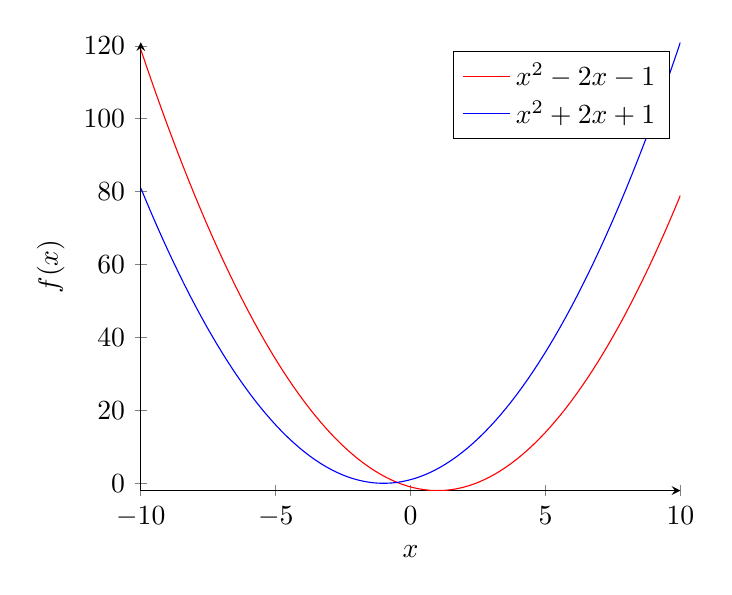
\begin{tikzpicture}
\begin{axis}[
    axis lines = left,
    xlabel = \(x\),
    ylabel = {\(f(x)\)},
]
%Below the red parabola is defined
\addplot [
    domain=-10:10, 
    samples=100, 
    color=red,
]
{x^2 - 2*x - 1};
\addlegendentry{\(x^2 - 2x - 1\)}
%Here the blue parabola is defined
\addplot [
    domain=-10:10, 
    samples=100, 
    color=blue,
    ]
    {x^2 + 2*x + 1};
\addlegendentry{\(x^2 + 2x + 1\)}

\end{axis}
\end{tikzpicture}
\end{center}
\caption{Un test avec pgfplot.}
\label{fig:test1}
\end{figure}


\begin{figure}[!t]
\begin{center}
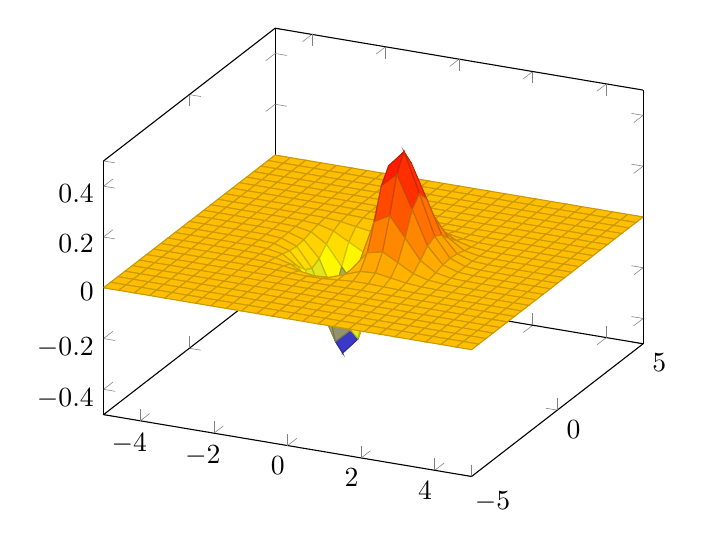
\begin{tikzpicture}
\begin{axis}
\addplot3[
    surf,
]
{exp(-x^2-y^2)*x};
\end{axis}
\end{tikzpicture}
\end{center}
\caption{Un autre test avec pgfplot.}
\label{fig:test2}
\end{figure}



\begin{figure}[!t]
\begin{center}
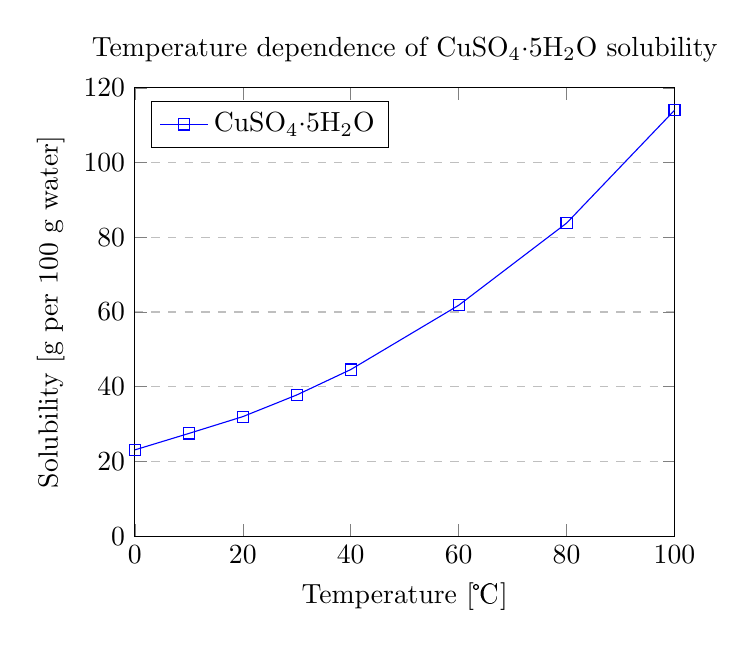
\begin{tikzpicture}
\begin{axis}[
    title={Temperature dependence of CuSO\(_4\cdot\)5H\(_2\)O solubility},
    xlabel={Temperature [\textcelsius]},
    ylabel={Solubility [g per 100 g water]},
    xmin=0, xmax=100,
    ymin=0, ymax=120,
    xtick={0,20,40,60,80,100},
    ytick={0,20,40,60,80,100,120},
    legend pos=north west,
    ymajorgrids=true,
    grid style=dashed,
]
\addplot[
    color=blue,
    mark=square,
    ]
    coordinates {
    (0,23.1)(10,27.5)(20,32)(30,37.8)(40,44.6)(60,61.8)(80,83.8)(100,114)
    };
    \legend{CuSO\(_4\cdot\)5H\(_2\)O}
\end{axis}
\end{tikzpicture}
\end{center}
\caption{Un graph de mesures avec pgfplot.}
\label{fig:test3}
\end{figure}


\begin{figure}[!t]
\begin{center}
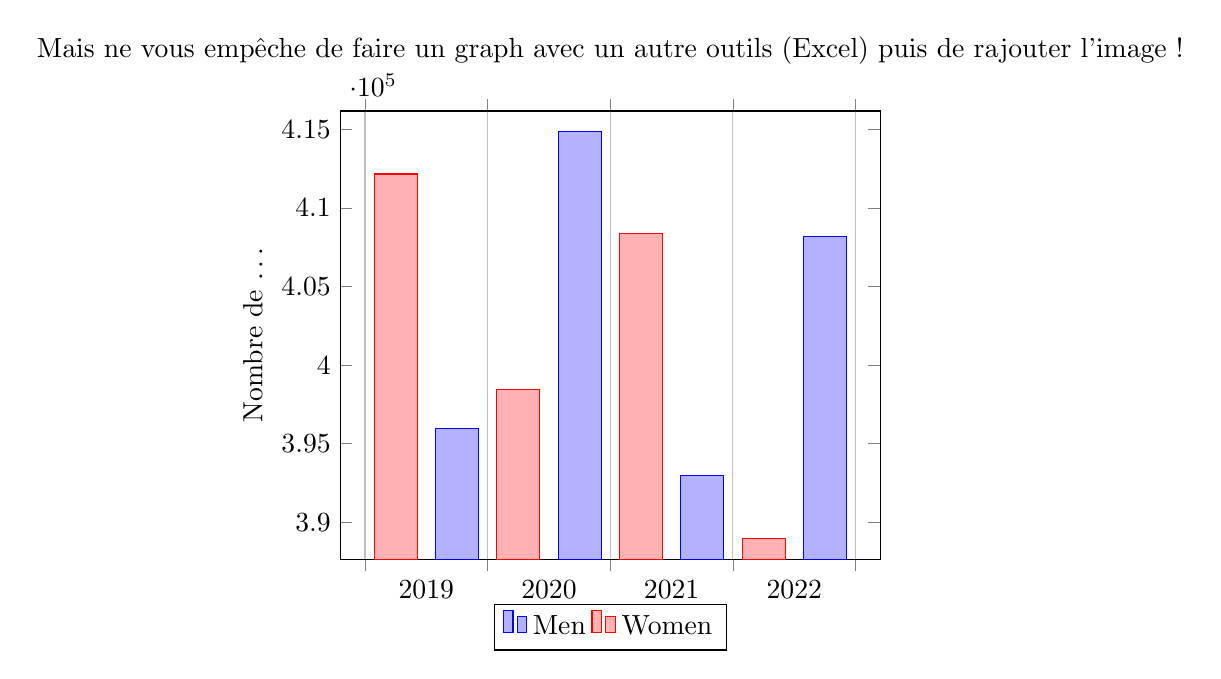
\begin{tikzpicture}
\begin{axis}[
title style={at={(0.5,1.15)},anchor=north},
title={Mais ne vous empêche de faire un graph avec un autre outils (Excel) puis de rajouter l'image !},
  x tick label style={
    /pgf/number format/1000 sep=},
  ylabel={Nombre de \( \ldots \) },
  xlabel=Années,
  enlargelimits=0.05,
  legend style={at={(0.5,-0.1)}, anchor=north, legend columns=-1},
  ybar interval=0.7,
]
%men
\addplot 
  coordinates { (2022,408184) (2021,393007) (2020,414870) (2019,395972) (2018,400000) }; %2018, bidon, juste affichage de 2019
%women
\addplot 
  coordinates { (2022,388950) (2021,408348) (2020,398449) (2019,412156) (2018,400000) }; %2018, bidon, juste affichage de 2019
\legend{Men,Women}
\end{axis}
\end{tikzpicture}
\end{center}
\caption{Un dernier graph avec pgfplot. }
\label{fig:test4}
\end{figure}
